\chapter{Termoaktivne lastnosti GPLA}\label{sec:PLA}
    
        Bistvena lastnost polilaktične kisline ali PLA (\textit{Polylactic acid}) je steklasti prehod iz trdnega v tekoče pri temperaturi steklenja $T_g$. Pri sobni temperaturi je PLA trd in krhek, z višanjem temperature preide v steklasto stanje (od $0,8 \, T_g$ do $T_g$) in nato v gumielastično področje (od $T_g$ do $1,4 \, T_g$), kjer se material z višanjem temperature mehča a plastično ne deformira. Pri ponovnem ohlajevanju se material povrne v prvotno stanje. Pri segrevanju nad $1,4 \, T_g$ material preide v plastično in nato talilno področje \cite{Glass_transition_Wiki}. Mehčanje materiala z višanjem temperature se izraža kot padanje modula elastičnosti $E$ oziroma togosti materiala, ki je temeljna karakteristika pri obravnavi dinamskih sistemov. Naš cilj je ugotoviti povezavo med modulom elastičnosti in temperaturo in preko nje krmiliti togost metamateriala. Eksperimentalno to dosežemo v poglavju \ref{sec:meritev_materialnih_lastnosti}. 
    
        Sprva torej potrebujemo mehanizem preko katerega bomo material lahko segrevali. Osnovnemu PLA-ju lahko z različnimi aditivi spremenimo lastnosti. V naši aplikaciji je bistvenega pomena dodatek grafitnega prahu, ki tvori GPLA (\textit{Graphite Polylactic acid}). Električna prevodnost grafita znatno zniža specifično upornost $\varrho$ GPLA-ja.
    
        Električni tok $I$ pri napetosti $U$, ki teče skozi dušilec z uporom: 
        \begin{equation}\label{eq:upor}
            R=\varrho\,l / A \, ,
        \end{equation}
        kjer je $A$ površina preseka in $l$ dolžina dušilca. Tok povzroča segrevanje zaradi Joulove moči $P=I^2R$. Upoštevamo konvekcijo in zapišemo energijski zakon \cite{Soft-Actuators_Al-Rubaiai}:
        \begin{align}\label{eq:energijska_bilanca}
            m \, c_p \frac{dT(t)}{dt}&=I^2R-h_s \, A_s \left( T(t)-T_\infty \right) \, ,
        \end{align}
        kjer je $m=\rho A l$ masa dušilca z gostoto $\rho$, $c_p=1600 \text{ J/kgK}$  specifična toplota materiala \cite{Thermal-properties-of-samples} in $A_s$ celotna površina v kontaktu z zrakom s koeficientom toplotne prestopnosti $h_s$. $T=T(t)$ je temperatura vzorca ob času $t$ in $T_\infty$ temperatura okolice, pri čemer je $T(t=0)=T_\infty$. Rešimo diferencialno enačbo \eqref{eq:energijska_bilanca}:
        \begin{equation}\label{eq:temperatura_analiticno}
            T(t)=T_\infty + \frac{A\,U^2 \left( 1-e^{-\frac{A_s h_s}{A c_p l \rho}\cdot t} \right)}{A_s h l \varrho} \, .
        \end{equation}
        Pokazali smo, da lahko z električnim tokom GPLA segrejemo. Z zgornjo enačbo analitično aproksimiramo potrebno električno napetost $U=\Delta V$, da v času $t$ dosežemo potrebno temperaturo. Kasneje v eksperimentalnem delu povežemo temperaturo z modulom elastičnosti, kar pomeni, da lahko preko električne napetosti, ki jo je dokaj enostavno nadzirati, krmilimo togost metamateriala. 
        
    \newpage
    \section{Meritev materialnih lastnosti GPLA-ja}\label{sec:meritev_materialnih_lastnosti}

        Preden se lotimo izdelave in analize metamateriala, moramo raziskati materialne lastnosti, ki so potrebne za njegovo dimenzioniranje in krmiljenje temperature z enačbo \eqref{eq:temperatura_analiticno}. Na podlagi meritev in analize vzorcev določimo gostoto $\rho$, specifično električno upornost $\varrho$ in modul elastičnosti $E$ GPLA-ja v odvisnosti od temperature. Eksperimente smo opravili v sklopu \cite{Bizjan_2021}.
        
        Materialne lastnosti FFF (\textit{Fused filament fabrication}) 3D tiskanih struktur so močno odvisne od parametrov izdelave. Vzorce (slika \ref{fig:vzorci}) smo modelirali v \textit{SolidWorks} CAD programu. Tiskamo z debelino sloja $0,2 \text{ mm}$ v smeri vzporedno dolžini ($0^\text{o}$) ali v smeri pravokotno na dolžino nosilcev ($90^\text{o}$) s $100\%$ polnitvijo. Dimenzije $a = 10\text{ mm}$, $b=5\text{ mm}$, $h=2\text{ mm}$ in $t=8\text{ mm}$ so konstantne, variiramo le dolžino $l$, ki je prvič $30 \text{ mm}$ in drugič $60\text{ mm}$. S kombinacijo smeri tiska in dolžin analiziramo štiri vzorce. Uporabimo filament proizvajalca \textit{ProtoPlant} na FFF 3D printerju \textit{Ultimaker 3}.
        \begin{figure}[!hb]
            \centering
            \includegraphics[width=0.70\textwidth]{slike/metodologija/vzorci.eps}
            \caption{Geometrija vzorcev za določanje materialnih lastnosti \cite{Bizjan_2021}.}\label{fig:vzorci}
        \end{figure}

            Gostota GPLA plastike $\rho=m/V$ je bila določena na podlagi pomerjene mase $m$ in na podlagi dimenzij vzorcev izračunanega volumna $V$. Za maso je bila uporabljena tehtnica EMB 200-3 proizvajalca KERN.
            
            Volumen prvega modela znaša $V_1=34708 \text{ mm}^3$ in masa $m_1=39,53 \text{ g}$. Za drugi model je volumen $V_2=35586 \text{ mm}^3$ in masa $m_2=36,33 \text{ g}$. Gostota prvega je tako $\rho_1=1107 \text{ kg/m}^3$ in drugega $\rho_2=1105 \text{ kg/m}^3$. Povprečna gostota vseh GPLA vzorcev pri $26^{\,\circ}$C je $\rho_{GPLA}=1106 \text{ kg/m}^3$.

            Vzorce opremimo tako, da omogočimo prevajanje toka in meritev temperature. Na mestu kontakta jih prebarvamo s srebrno prevodno barvo in prelepimo s tanko bakreno žico. Na sredini namestimo termočlen tipa K, ki je sposoben meriti temperaturo od 0 do 100 $^o$C. Vzorec je del električnega merilnega vezja in deluje kot upor (slika \ref{fig:merilna_shema_a}). Padec napetosti $U$ merimo preko delilnika napetosti $U_{out}$. Tok $I$ lahko določimo z uporabo upora znane in dovolj majhne vrednosti, na katerem izmerimo napetost $U_{shunt}$. Meritev na delilniku in \textit{shuntu} pretvorimo v napetost in tok na vzorcu prek izrazov:
            \begin{align}
                U &= \frac{U_{out}}{0,09007}-U_{shunt} \,, \\
                I&=\frac{U_{shunt}}{1,1 \, \Omega} \, .
            \end{align}
            
            Temperaturo merimo na merilni kartici NI 9211, tok in napetost pa na NI 9215. Priključeni sta na računalnik, na katerem meritve analiziramo s programom \textit{LabView}. Specifično električno upornost $\varrho$ določimo z Ohmovim zakonom $R=U /I$ in enačbo \eqref{eq:upor} ter jo prikažemo v spodnjem grafu \ref{fig:spec_el_upornost}. Vidimo, da s temperaturo upornost narašča.
            \begin{figure}[!htb]
                \centering
                \begin{subfigure}{.489\textwidth}
                    \centering
                    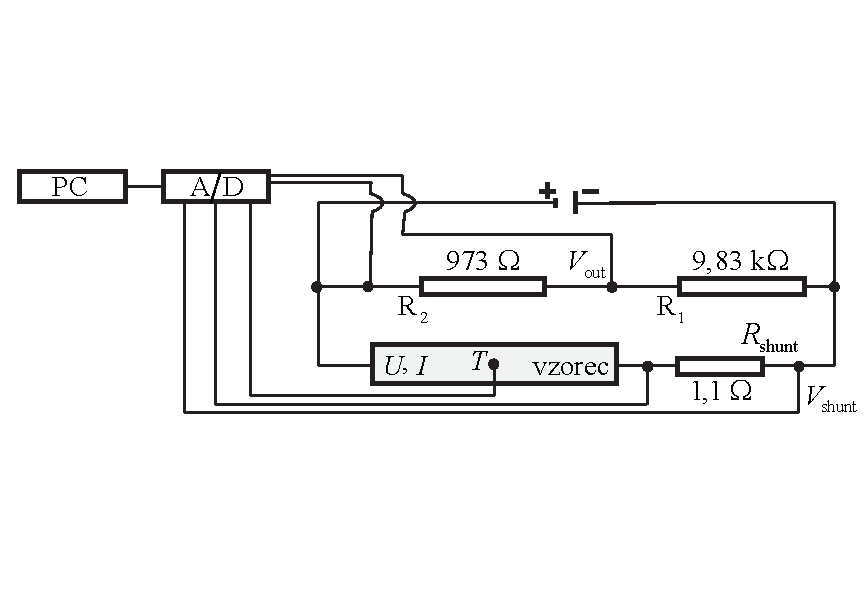
\includegraphics[width=\linewidth]{Magisterski praktikum/slike/metodologija/vezje.pdf}
                    \caption{}
                    \label{fig:merilna_shema_a}
                \end{subfigure}%
                \begin{subfigure}{.489\textwidth}
                    \centering
                    \includegraphics[trim={0.5cm 0cm 2.5cm 2cm}, clip, width=\linewidth]{Magisterski praktikum/slike/metodologija/specifična_upornost.pdf}
                    \caption{}
                    \label{fig:spec_el_upornost}
                \end{subfigure}%
                \caption{(a) Shema vezja meritve in (b) specifična upornost $\varrho$ GPLA materiala \cite{Bizjan_2021}.}
                \label{fig:merilna_shema}
            \end{figure}
            Določimo modul elastičnosti GPLA-ja ter njegovo odvisnost od temperature. Predstavimo metodo določanja modula elastičnosti materiala prek identifikacije lastne frekvence in geometrije strukture \cite{Pintelon_2003}, \cite{Kosir_2021}, ki jo analiziramo z MKE.
            Predpostavimo Hookov zakon, oziroma z drugimi besedami linearno teorijo elastičnosti, in frekvenčno neodvisnost materiala. Obravnavano geometrijo strukture rešujemo z analizo lastnih frekvenc po MKE. Izhajamo iz enačbe \ref{eq:karakteristica_en}, kjer matrike $[A\,]=[K][M^{-1}]$ vsebujejo modul elastičnosti $E$, Poissonov količnik $\nu$ in gostoto $\rho$:
            \begin{align}
                [K]&=E \, [K_0] \,,\\
                [M]&=\rho \, [M_0]\,.
            \end{align}
            $[K_0]$ predstavlja togostno matriko neodvisno od modula elastičnosti $E$ in $[M_0]$ masno matriko neodvisno od gostote $\rho$. $[K_0]$ ni povsem odvisna le od geometrije strukture, saj je še vedno odvisna od Poissonovega količnika $\nu$. Vendar če se omejimo na strukture, ki jih lahko obravnavamo kot Euler-Bernoullijev nosilec \cite{rao2007ContinuousSystems}, je $\nu$ zanemarljiv in $[K_0]$ materialno neodvisna matrika. Sistem enačb \eqref{eq:karakteristica_en}, kjer je $\lambda=\omega^2$:
            \begin{align}
                \left(\,[A\,] - \omega^2 \, [\,I\,] \, \right) \vv{\overline{Q}}&=\vv 0 \nonumber \,,\\
                \left(\,[K][M^{-1}] - \omega^2 \, [\,I\,] \, \right) \vv{\overline{Q}}&=\vv 0 \nonumber \,,\\
                \left(\,[K] - \omega^2 \, [M] \, \, \right) \vv{\overline{Q}}&=\vv 0 \nonumber \,,\\
                \left(\,E \, [K_0]-\omega^2 \rho \, [M_0] \, \right) \vv{\overline{Q}}&=\vv 0 \nonumber \,,\\
                \left( \, [K_0]-\omega^2 \frac{\rho}{E} \, [\,I\,] \, \right) \vv{\overline{Q}}&=\vv 0 \,,\nonumber
            \end{align}
            preoblikujemo v nov problem lastnih vrednosti z $\lambda=\omega^2 \rho / E$:
            \begin{align}
                \left( \, [K_0]- \lambda \, [\,I\,] \, \right) \vv{\overline{Q}}&=\vv 0 \,.
            \end{align}
            
            Materialno neodvisni lastni problem uporabimo za izračun $i$-te lastne vrednosti po MKE, ki jo povežemo z eksperimentalno izmerjeno $i$-to lastno frekvenco $f_{0,i}$, kot je definirana v enačbi \eqref{eq:lastna_frekvenca}.
            Tako je:
            \begin{align}\label{eq:karakteristica_en_modul}
                \lambda_i = 4 \pi^2 \frac{\rho}{E} f_{oi}^2 \,.
            \end{align}
            Za določanje efektivnega modula elastičnosti $E$ v nadaljevanju potrebujemo gostoto $\rho$, pomerjeno prvo lastno frekvenco $f_{0,1}$ ter po MKE izračunano prvo lastno vrednost $\lambda_1$. Na podlagi enačbe \eqref{eq:karakteristica_en_modul} lahko določimo modul elastičnosti $E$ kot:
            \begin{equation}\label{eq:modul}
                E=4 \pi^{2} \, \frac{\rho \, f_{0,1}^{2}}{\lambda_{1}} \, .
            \end{equation}
            V naslednjem koraku vzorce na mestu izoliranih (belih PLA) površin s sekundnim lepilom pritrdimo na ploščo stresalnika LDS V555 (slika \ref{fig:merilna_shema_2}). Nanjo smo namestili referenčni pospeškomer proizvajalca PCB Piezotronics, ki je povezan na tretjo merilno kartico NI 9234, na kateri je tudi laserski merilnik hitrosti Polytec PDV 100 (slika \ref{fig:merilna_shema_1}). Sedaj izvedemo modalno analizo testiranih vzorcev z MKE v programu \textit{ANSYS Mechanical} \cite{thompson2017ansys}. Poissonov količnik je privzet iz literature in znaša $\nu = 0,39$ \cite{Ferreira_2017}. Za vsak vzorec določimo matriki $[K_0]$, $[M_0]$ ter rešimo problem lastnega nihanja po enačbi \eqref{eq:karakteristica_en_modul} in izračunamo prvo lastno vrednost $\lambda_1$ (slika \ref{fig:MKE_vzorca}).
            \begin{figure}[!htb]
            \centering
            \tabskip=0pt
            \valign{#\cr
              \hbox{%
                \begin{subfigure}[b]{.45\textwidth}
                \centering
                \includegraphics[height=11cm, width=\textwidth]{Magisterski praktikum/slike/metodologija/merino_mesto_1.png}
                \caption{}
                \label{fig:merilna_shema_1}
                \end{subfigure}%
              }\cr
              \noalign{\hfill}
              \hbox{%
                \begin{subfigure}{.45\textwidth}
                \centering
                \includegraphics[height=5.0cm, width=\textwidth]{Magisterski praktikum/slike/metodologija/merino_mesto_2.png}
                \caption{}
                \label{fig:merilna_shema_2}
                \end{subfigure}%
              }\vfill
              \hbox{%
                \begin{subfigure}{.45\textwidth}
                \centering
                \includegraphics[height=4.5cm,width=\textwidth]{Magisterski praktikum/slike/metodologija/MKE_E_modul.png}
                \caption{}
                \label{fig:MKE_vzorca}
                \end{subfigure}%
              }\cr
            }
            \caption{Prikaz (a) eksperimenta za meritev modula elastičnosti (b) GPLA vzorca in (c) njegovega MKE modela za analizo lastnih vrednosti.}
            \end{figure}
            
            
            \newpage
            
            Vzorce smo vzbujali z belim šumom s konstantno amplitudo pospeška na frekvenčnem razponu od 40 do 1000 Hz. S pomerjenimi signali pospeška in hitrosti smo določili amplitudni del frekvenčne prenosne funkcije FPF vsakega vzorca pri različnih temperaturah in prvo lastno frekvenco $f_{0,1}$ (slika \ref{fig:merilna_shema_b}).  
            
            Z uporabo enačbe \eqref{eq:modul} določimo ekvivalentni modul elastičnosti GPLA materiala $E=E(T)$ in ga predstavimo v spodnjem grafu \ref{fig:modul_elastičnosti} ter določimo temperaturo steklenja $T_g=45 ^\text{ o}$C v primeru printanja pri orientaciji $0^\text{o}$. Pri tej temperaturi postane struktura stalno deformirana zaradi pričetka taljenja in se z ohlajanjem ne povrne v prvotno stanje. 
            
            Modul elastičnosti $E_{GPLA}(22^\text{ o}\text{C})=2400\text{ MPa}$ in $E_{GPLA}(42^\text{ o}\text{C})=2000\text{ MPa}$ pri orientaciji $0^\text{o}$ in  $E_{GPLA}(22^\text{ o}\text{C})=2100\text{ MPa}$ in $E_{GPLA}(35^\text{ o}\text{C})=1900\text{ MPa}$ pri orientaciji $90^\text{o}$. V nadaljevanju bomo metamaterial modelriali z uporabo kota printanja $0^\text{o}$.
            
            Tako smo določili gostoto $\rho$ in modul elastičnosti $E$, ki sta potrebni za modeliranje metamateriala, kar je naslednji korak raziskave.
            
            \begin{figure}[!htb]
                \centering
                \begin{subfigure}{.70\textwidth}
                    \centering
                    \includegraphics[width=\linewidth]{Magisterski praktikum/slike/metodologija/FRF.pdf}
                    \caption{}
                    \label{fig:merilna_shema_b}
                \end{subfigure}
                \begin{subfigure}{.70\textwidth}
                    \centering
                    \includegraphics[trim={0.0cm 0cm 2.5cm 2cm}, clip, width=\linewidth]{Magisterski praktikum/slike/metodologija/modul_elastičnosti.pdf}
                    \caption{}
                    \label{fig:modul_elastičnosti}
                \end{subfigure}
                \caption{(a) Shema vezja meritve, (b) FPF vzorca $l=60$ in $0^\circ$, (c) specifična upornost $\varrho$ in (d) modul elastičnosti $E$ GPLA pri različnih temperaturah \cite{Bizjan_2021}.}
            \end{figure}
        
